% !TEX root=./index.tex

\section{Abstract}
\begin{abstract}
	This report focuses on the phenomenons encountered in the simulation of a simple full adder, to reveal some critical features of FPGA programming comparing to ordinary programmable devices. Among these phenomenons, jitters and the race-hazard conditions are of the most concerns.
\end{abstract}

\section{Introduction}

Half adder and full adder are basic elements in digital circuits used to perform addition operations on binary numbers.

A half adder

\begin{figure}[htpb]
	\begin{center}
		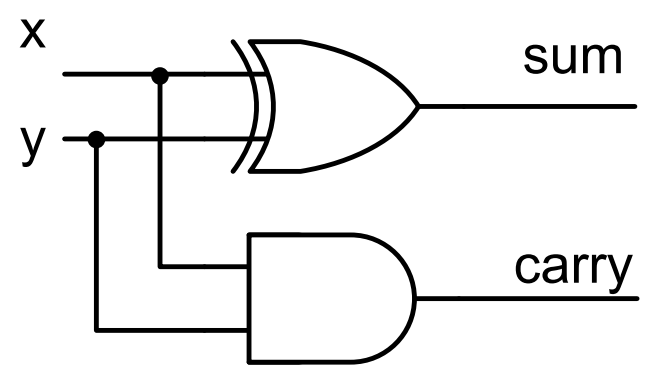
\includegraphics[width=0.22\textwidth]{index.assets/20240303235723.png}
		\caption{Gate Level Description of Half Adder}
	\end{center}
\end{figure}

is a combinational logic circuit that takes two binary inputs and produces two binary outputs: sum and carry.

\begin{eqnarray}
	\mathop{\mathrm{HA}}:(x_1,x_2)\mapsto(Q,C) :=
	\begin{cases}
			Q&=\mathop{\mathrm{xor}}(x_1,x_2) \\
			C&=\mathop{\mathrm{and}}(x_1,x_2)
	\end{cases}
\end{eqnarray}

The main limitation of the half adder is that it cannot handle carry inputs and therefore can only be used for 1-bit addition.

A full adder

\begin{figure}[htpb]
	\begin{center}
		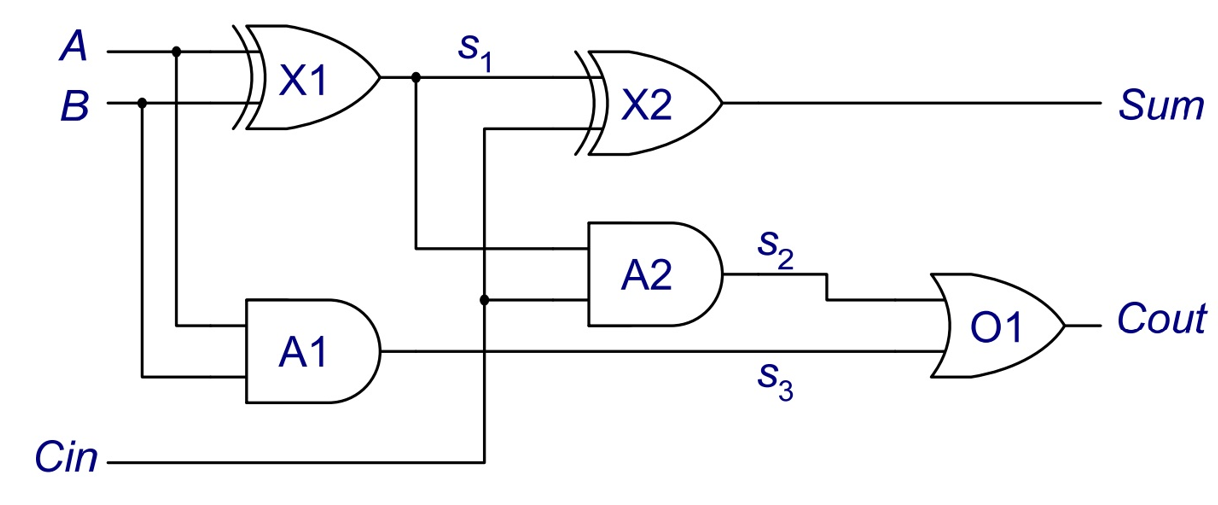
\includegraphics[width=0.45\textwidth]{index.assets/20240303235337.png}
		\caption{Gate Level Description of Full Adder}
	\end{center}
\end{figure}\label{FA_GateLevel}

is an extension of the half adder that accepts three binary inputs: two additions and a rounding input, and produces two binary outputs: sum and carry. Full adders can be connected in series to achieve binary addition of any number of bits.

Implementation of full adder can be derived directly from 3-digit addition, where the final carry output is toggled if any of \(X_1+X_2\) or \(C_i+Q_1\) produces a carry:

\begin{eqnarray}
	(q_1,c_1)&=\mathop{\mathrm{HA}}(x_1,x_2) \\
	(q_2,c_2)&=\mathop{\mathrm{HA}}(q_1,c_i) \\
	c_o &= \mathop{\mathrm{or}}(c_1,c_2)
\end{eqnarray}

Therefore the gate-level circuit of the full adder can be easily captured, as shown of Figure. (\ref{FA_GateLevel})
